\chapter{Querschnittliche Konzepte}
\label{sec:quer}

Bei der Entwicklung und Umsetzung einer Architektur gibt es mehrere Konzepte die an mehreren Stellen berücksichtigt werden sollten. Diese Konzepte werden daher auch als querschnittliche Konzepte bezeichnet. Für das Projekt eCourse sind diese Konzepte in Abbildung \ref{fib:querschnitt}dargestellt.


\begin{landscape}
\begin{figure}[H]
\centering
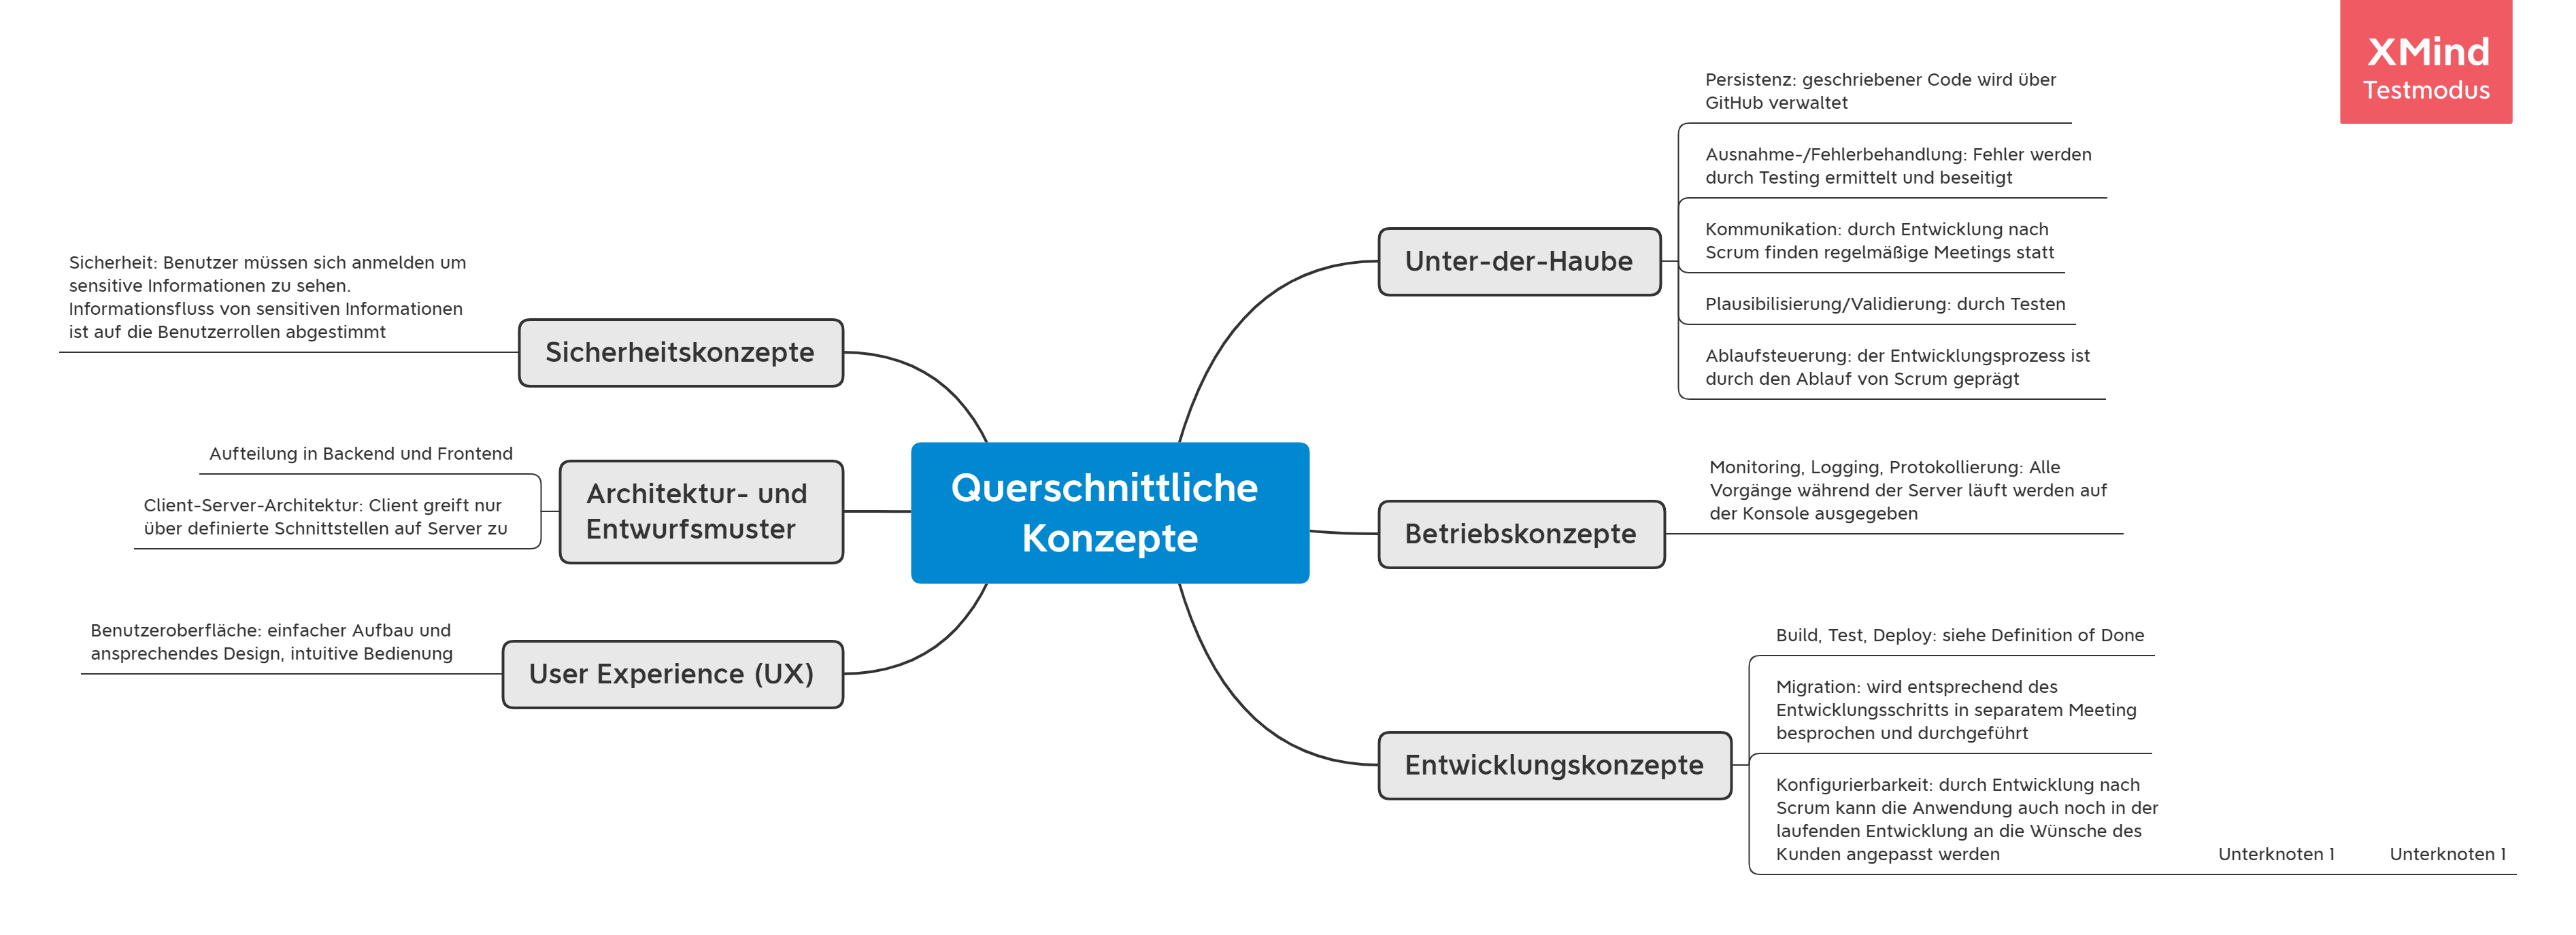
\includegraphics[height=0.6\textwidth]{querschnittliche_konzepte.png}
\caption{Querschnittliche Konzepte die zur Entwicklung von eCourse beitragen}
\label{fib:querschnitt}
\end{figure}
\end{landscape}
